\documentclass{beamer}

\usepackage{url}
\usepackage{tikz}
\usetheme{Madrid}

\title{Julia for Linear Programming}
\author{Iain Dunning and Miles Lubin}
\date{IAP -- January 16, 2013}
\institute{MIT}

\setbeamercovered{invisible}
\setbeamertemplate{navigation symbols}{}
\setbeamertemplate{footline}[page number]

\begin{document}

\frame{\titlepage}

\begin{frame}
	\frametitle{What is Linear Programming (LP)}
	\begin{align*}
		\text{Maximize}   \quad & c^T x \quad \text{over } x \in \mathbb{R}^N \\
		\text{Subject to} \quad & a^T_i x \leq b_i \quad \forall i=1,\ldots,M
	\end{align*}
	\begin{itemize}
		\item Widely used - airline scheduling, production planning, TeX hyphenation...
		\item Simplex algorithm for LP named in "Top 10 Algo. of 20th Century" by SIAM
	\end{itemize}
\end{frame}

\begin{frame}[fragile]
	\frametitle{How are they solved - Modeling}
	\begin{itemize}
		\item Why use modeling languages?
	\end{itemize}
    \begin{verbatim}
    maximize Obj:
      sum {j in 1..N} profit[j] * x[j];
	  
    subject to CapacityCons:
      sum {j in 1..N} weight[j] * x[j] <= Capacity;
	\end{verbatim}
	\begin{itemize}
		\item Options
		\begin{itemize}
			\item Commercial - e.g. AMPL, GAMS
				\begin{itemize}
					\item Specialized - so fast
					\item Not general purpose language
				\end{itemize}
			\item Open-source - e.g. PuLP, Pyomo, CVX, YALMIP
				\begin{itemize}
					\item Built on Python or MATLAB
					\item Use operator overloading - slower
				\end{itemize}
		\end{itemize}
	\end{itemize}
\end{frame}

\begin{frame}[fragile]
	\frametitle{Modeling in Julia}
	\begin{center}
		\url{http://github.com/IainNZ/Julp}
	\end{center}
	\begin{itemize}
		\item Julia replaces domain-specific language
		\item Use macros to avoid issues with operator overloading
	\end{itemize}
	{\small
	\begin{verbatim}
    m = Model("max")
    x = [ Variable(m) for j = 1:N ]
    profit = rand(N);  weight = rand(N);
    
    setObjective(m, 
        @sumExpr([ profit[j] * x[j] for j = 1:N ])
    )
    
    addConstraint(m,
        @sumExpr([ weight[j] * x[j] for j = 1:N ])
    )
	\end{verbatim}
	}
\end{frame}

\begin{frame}[fragile]
	\frametitle{Macro and Benchmark}
	\begin{itemize}
		\item Macro only 3 (long-ish) lines
		\item Breaks \texttt{[c[i] * x[i] for i = 1:N]} into...
		\begin{itemize}
			\item \texttt{[c[i] for i = 1:N]}
			\item \texttt{[x[i] for i = 1:N]}
		\end{itemize}
		\item ... which is how constraints are stored
		\item Benchmark times (in seconds):
	\end{itemize}
	\begin{table}
		\begin{tabular}{|c|c|c|}
			\hline
			Lang. & N=5000 & N=10000 \\
			\hline
			AMPL & 4 & 6 \\
			Julia (Julp) & 6.44 & 16.29 \\
			PyPy2 (PuLP) & 26.62 & 53.45 \\
			Python (PuLP) & 111.80 & 222.95 \\
			\hline
		\end{tabular}
	\end{table}
\end{frame}

\begin{frame}
	\frametitle{How are they solved -- Algorithms}
	\begin{itemize}
		\item Dantzig's simplex algorithm most used method.
		\item Computationally very challenging to implement efficiently
		\begin{itemize}
			\item Naturally not vectorizable -- specialized sparse linear algebra
			\item Typically memory bound -- cache misses
		\end{itemize}
		\item Matlab implementations too slow to be used in practice
		\begin{itemize}
			\item High-quality open-source codes exist in C++
		\end{itemize}
		\item Can Julia compete?
	\end{itemize}
\end{frame}

\begin{frame}
	\frametitle{Simplex Benchmarks}
	\begin{center}
		\url{https://github.com/mlubin/SimplexBenchmarks}
	\end{center}
	\begin{itemize}
		\item Benchmark of some important operations:
	\end{itemize}
\begin{table}\begin{center}
\begin{tabular}{|c|c|c|c|c|c|c|}
\hline
		       & Julia  & C++  &   C++bnd  &Matlab & PyPy &   Python  \\
\hline
Sp.\ mat-sp.\ vec& 1.29  &  0.90  &  1.00  &  5.79 &   19.20 &  417.16\\ 
Sp.\ vector scan &  1.59  &  0.96 &   1.00  &  13.98 &  13.81 &  48.39\\
Sp.\ \texttt{axpy}& 1.85  &  0.70  &  1.00  &  19.12  & 9.21  &  78.65\\
\hline
\end{tabular}\end{center}
\end{table}
	\begin{itemize}
		\item C++bnd = C++ with bounds checking
		\item Execution times relative to C++bnd
	\end{itemize}
\end{frame}

\begin{frame}
	\frametitle{Tutorial}
	\begin{center}
		\url{https://github.com/JuliaLang/IAP2013/blob/master/NumericalOptimization/tutorial.pdf}
	
	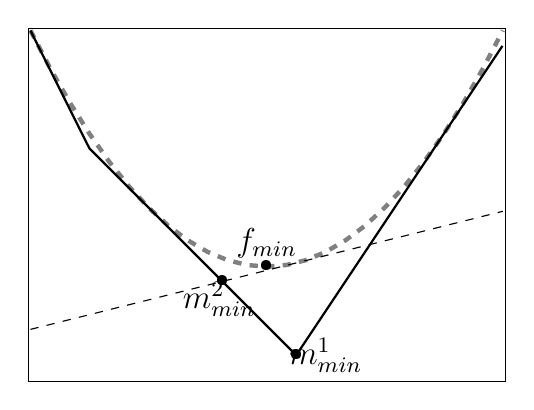
\begin{tikzpicture}[xscale=3,yscale=6]
\draw [gray,ultra thick,dashed,domain=0:2] plot (\x, {0.5*(\x-1)^2});
%\draw [dashed,domain=0:1] plot (\x, {-1*\x + 0.5});
%\draw [dashed,domain=0:2] plot (\x, {-\x/2 + 3/8});
%\draw [dashed,domain=1:2] plot (\x, {(3/4)*\x-1.03125});
\draw [thick,domain=0:2,samples=200] plot (\x, {max(-1*\x + 0.5,max(-\x/2 + 3/8,(3/4)*\x-1.03125))});
\node () at (1,0) {\textbullet};
\node [font=\large] () at (1,0.05) {$f_\text{min}$};
\node () at (1.125,-0.1875) {\textbullet};
\node [font=\large] () at (1.25,-0.1875) {$m_\text{min}^1$};
\draw [dashed,domain=0:2] plot (\x, {0.125*\x - 0.132813});
\node () at (0.812501,-0.0312504) {\textbullet};
\node [font=\large] () at (0.8,-0.07) {$m_\text{min}^2$};
\draw (current bounding box.north east) rectangle (current bounding box.south west);
\end{tikzpicture}\end{center}
	\begin{itemize}
	\item Tutorial for implementing a parallel asynchronous optimization algorithm in Julia using master-worker paradigm
	\item No background in optimization needed
	\end{itemize}

\end{frame}

\end{document}
